\documentclass[a4paper, 12pt]{article}
\usepackage[a4paper,top=1.5cm, bottom=1.5cm, left=1cm, right=1cm]{geometry}

% Работа с русским языком
\usepackage[utf8]{inputenc}
\usepackage{mathtext}                % русские буквы в формулах
\usepackage[english, russian]{babel} % локализация и переносы

\usepackage{graphicx}   % Вставка изображений
\usepackage{float}      % "Плавающие" изображения3
\usepackage{wrapfig}    % Обтекание фигур (таблиц, картинок и прочего)
\usepackage{subfig}
\graphicspath{ {./images/} }

\usepackage{tabularx}
\usepackage{multirow}
\usepackage{booktabs}
\usepackage{amsmath}
\usepackage{amsfonts}
\usepackage{indentfirst}
\usepackage{longtable}
\graphicspath{{pictures/}}
\usepackage{natbib}
\usepackage{bm}

\newcommand{\figref}[1]{(См. рис. \ref{#1})}
\newcommand{\secref}[1]{(См. раздел. \ref{#1})}


%%% Колонтитулы
\usepackage{titleps}
\newpagestyle{main}{
	\setheadrule{0.4pt}
	\sethead{Отчёт о выполнении лабораторной работы 10.1}{}{}
	\setfootrule{0.4pt}                       
	\setfoot{ФРКТ МФТИ, 2024}{}{\thepage} 
}
\pagestyle{main}  

\begin{document}
    \begin{titlepage}
	\begin{center}
            {\large МОСКОВСКИЙ ФИЗИКО-ТЕХНИЧЕСКИЙ ИНСТИТУТ (НАЦИОНАЛЬНЫЙ ИССЛЕДОВАТЕЛЬСКИЙ УНИВЕРСИТЕТ)}
	\end{center}
 
	\begin{center}
		{\large Физтех-школа радиотехники и компьютерных технологий}
	\end{center}
	
	\vspace{8cm}
	{\LARGE
		\begin{center}
                {\bf Отчёт о выполнении лабораторной работы 10.1}\\
                Электронный парамагнитный резонанс
		\end{center}
	}
	\vspace{4cm}
	\begin{flushright}
		{\Large Авторы: \\ 
        Тихонов Дмитрий Романович, \\ студент группы Б01-206а \\
        Павловский Кирилл Михайлович, \\ студент группы Б01-206а}
	\end{flushright}
	\vspace{4cm}
	\begin{center}
		\Large Долгопрудный, 2024
	\end{center}
    \end{titlepage}


    \section{Введение}

    \noindent \textbf{Цель работы:} исследовать электронный парамагнитный резонанс в молекуле ДФПГ; определить $g$-фактор электрона; измерить ширину линии ЭПР. \\
	

    \noindent \textbf{В работе используются:} осциллограф INSTEK GDS-620, фазовращатель, трансформатор ЛАТР, вольтметры GDM-8145, источник постоянного тока GRP-30H10D, частотомер GFC-8010H, генератор ВЧ Г4-116, основные катушки, модуляционные катушки, пробная катушка.
    
    \section{Теоретические сведения}

    Энергетический уровень электрона в присутствии магнитного поля с индукцией $B$ расщепляется на два подуровня, расстояние между которыми равно

    \begin{equation}
        \Delta E = 2\mu B_0,
        \label{eq:frequency_value}
    \end{equation}

    где $\mu$ -- абсолютная величина проекции магнитного момента на направление поля.

    Между этими двумя уровнями возможны переходы. Эти переходы могут возбуждаться внешними высокочастотным электромагнитным полем, если оно имеет нужную частоту и нужное направление.

    Резонансное значение частоты определяется из очевидной формулы:

    $$
    \hbar \omega_0 = \Delta E.
    $$

    При переходе с нижнего на верхний уровень энергии электрон поглощает квант электромагнитной энергии, а при обратном переходе такой же квант излучается. Возбуждение электронных резонансных переходов электромагнитным полем, имеющим частоту $\omega_0$, носит название электронного парамагнитного резонанса (ЭПР).
    
    В настоящей работе необходимо получить сигнал ЭПР на кристаллическом дифенилпикрилгидразиле (ДФПГ) и определить значение $g$-фактора для электрона. Как известно, связь между магнитным моментом $\mu$ электрона и его механическим моментом $\mathbf{M}$ выражается через гиромагнитное отношение $\gamma$ с помощью формулы

    $$
    \mu = \gamma M.
    $$
    
    Если магнитный момент частицы измерять в магнетонах Бора, а механический - в $\hbar$, то их связь можно записать через $g$-фактор:
    $$
    \frac{\mu}{\mu_\text{Б}} = g \frac{M}{\hbar} = g \frac{s \hbar}{\hbar} = gs = \frac{\hbar \omega_0}{2 B_0 \mu_\text{Б}},
    $$
    
    где $s = \frac{1}{2}$ -– спин электрона. Следовательно, $g$ - фактор равен

    $$
    g = \frac{\hbar \omega_0}{\mu_\text{Б} B_0}.
    $$
    
    \newpage
    
    \section{Методика измерений и экспериментальная установка}

    \subsection{Описание экспериментальной установки}

    Схема экспериментальной установки приведена на рис. \ref{fig:installation}.

    \begin{figure}[H]
        \centering
        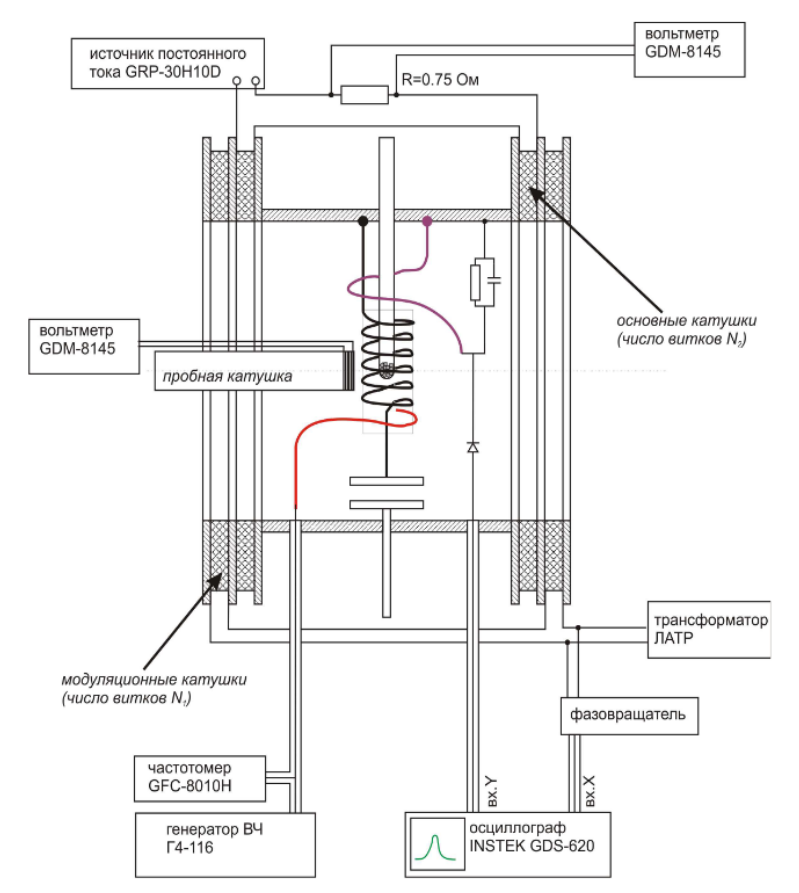
\includegraphics[width = 0.5\linewidth]{images/installation.png}
        \caption{Блок-схема экспериментальной установки}
        \label{fig:installation}
    \end{figure}

    \subsection{Оборудование и приборы}

    \begin{itemize}
        \item Цифровые мультиметры GDM-8145. В режиме измерения постоянного напряжения погрешность измерения оценивается по формуле 
        
        $$
        \pm (0.03\% \cdot \text{<измеренное значение>} + 4 \text{ единицы младшего разряда}).
        $$
        
        В режиме измерения постоянной силы тока на пределе $20 \A$ допустимое отклонение измеренных значений от реальных составляет 
        $$
        \pm (0.3\% \cdot \text{<измеренное значение>} + 2\text{ единицы младшего разряда}).
        $$
    \end{itemize}
	
    \subsection{Методика эксперимента}

     Для наблюдения электронного парамагнитного резонанса нужно поместить исследуемое вещество в магнитное поле и измерить поглощение электромагнитного излучения, частота которого удовлетворяет соотношению \ref{eq:frequency_value}. Поглощение, связанное с электронным парамагнитным резонансом, очень мало. Заметный эффект удается получить, применяя колебательный контур, который сосредотачивает энергию электромагнитного поля в объеме образца, помещенного в катушку. 
    \newpage
	
    \section{Результаты измерений и обработка данных}

    \subsection{Получение сигнала ЭПР на свободном радикале ДФПГ и измерение $g$-фактора электрона}
    
    Включим и настроим генератор и осциллограф, получим на экране картину модулированных колебаний. Включим питание основных катушек от источника постоянного тока и питание модулирующих катушек -- через автотрансформатор -- от сети переменного тока $220$ В. Установим на модулирующих катушках напряжение около $50$ В. Плавно меняя реостатом величину тока, проходящего через основные катушки, найдём сигнал ЭПР. Отрегулируем величину тока так, чтобы расстояние между пиками резонанса на экране осциллографа было одинаковым (см. рис. \ref{img:peaks}).

    \begin{figure}[H]
    	\centering
    	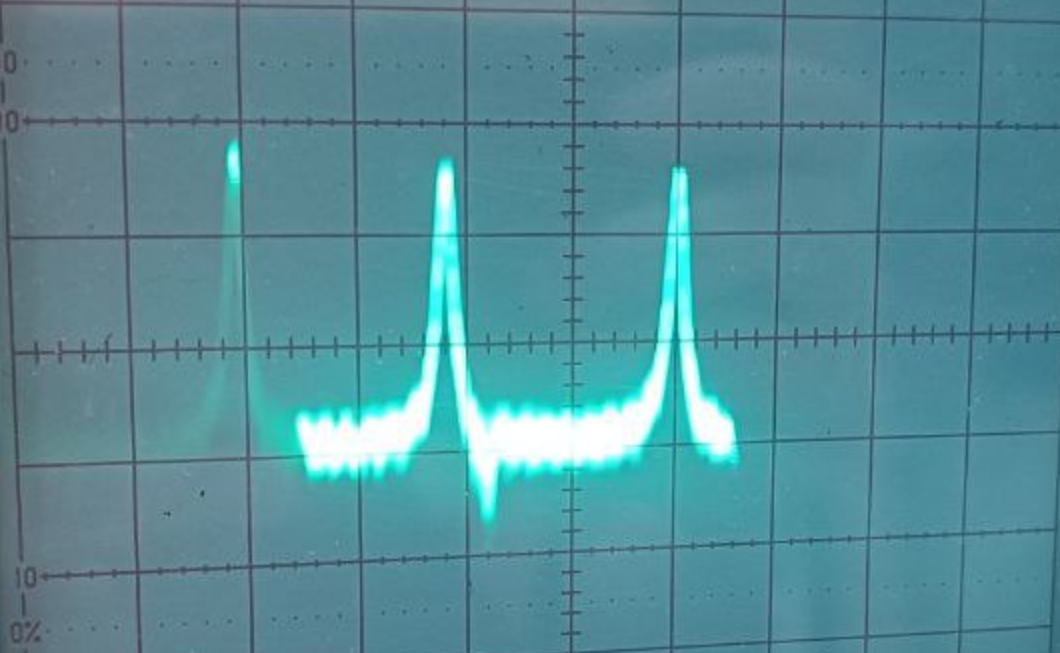
\includegraphics[width = 14 cm]{images/peaks.png}
        \caption{Пики резонанса на экране осциллографа}
        \label{img:peaks}
    \end{figure}

    Включим вилку питания пробной катушки в клеммы автотрансформатора. Измерим величину переменного поля. Для этого введём пробную катушку внутрь основных катушек поблизости от образца и запишем показания вольтметра: $V = \left( 11.6 \pm 0.5 \right) \text{ мВ}$. Зная число витков ($n = 45$) и площадь сечения ($S = \frac{\pi D^2}{4} = \frac{3.14 \cdot (14.5 \cdot 10^{-3})^2}{4} = \left( 1.65 \pm 0.08 \right) \cdot 10^{-4} \text{ м}^2$) пробной катушки, определим напряжённость поля:

    $$
    B_0 = \frac{V}{nS \cdot 2\pi\nu_{net}} = \left(5.0 \pm 0.3 \right) \text{ мТл}
    $$

    Теперь вычислим $g$-фактор электрона, зная, что частота резонанса равна \(\omega_0 = \left( 140.1 \pm 0.1 \right) \text{ МГц}\):
    $$
    g = \frac{\hbar\omega_0}{\mu_{\text{Б}}B_0} = \left( 2.0 \pm 0.1 \right) 
    $$

    \subsection{Определение ширины линии ЭПР}
    
    Получив сигнал ЭПР на ДФПГ в прошлом пункте, переключим осциллограф с временной развёртки на развёртку от модуляционных катушек.

    \begin{figure}[H]
        \centering
        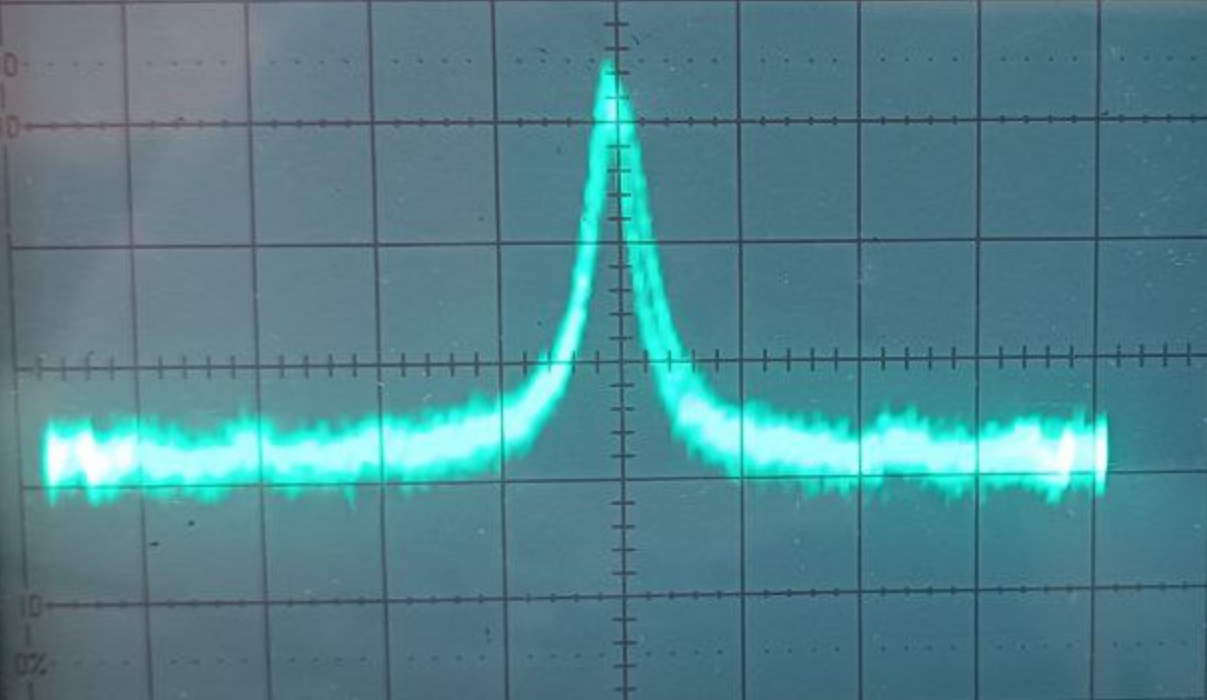
\includegraphics[width = 14 cm]{images/osc_X_Y.png}
        \caption{Сигналы поглощения электронного парамагнитного резонанса при развертке луча осциллографа напряжением моделирующих катушек}
        \label{img:osc_X_Y}
    \end{figure}

    Для определения ширины линии ЭПР определим по экрану осциллографа полный размах поля $A_0$ и полную ширину кривой резонансного поглощения на полувысоте $A_{1/2}$:

    $$
    A_0 = \left( 9.0 \pm 0.2 \right) \text{ дел.}, \: A_0 = \left( 0.4 \pm 0.2 \right) \text{ дел.}.
    $$
    
    При этом амплитуда поля измеряется так же, как и в первом пункте: 
    $$
    B_0 = \left(5.0 \pm 0.3 \right) \text{ мТл}.
    $$

    Отсюда, получим ширину линии ЭПР:

    $$
    \Delta B = \frac{A_{1/2}}{A_0} B_0 \approx 0.2 \text{ мТл} \approx 2 \text{ Гс}.
    $$
    
    \section{Заключение}
    
    \begin{itemize}
        \item Было экспериментально получено значение $g$-фактора электрона $g = \left( 2.0 \pm 0.1 \right)$. Полученное значение совпадает с теоретическим ($g = 2$), значит ЭПР происходит на неспаренных электронах почти так же, как и на свободных.

        \item Ширина линии дифенилпикрилгидразила составляет около 2 Гс, что также совпадает с теоретическим значением.

    \end{itemize}
    
\end{document}